\documentclass{CSIM}
\usepackage{graphicx}
\usepackage{enumitem}
\usepackage{subcaption}
\usepackage{hyperref} % Added for email links on the title page
\usepackage{amsmath}
\usepackage{cleveref}

\graphicspath{{./img/}}
\begin{document}

% Includes project title, team members, course, instructor, date, and subtitle placeholder.
\begin{titlepage}
    \centering
    \vspace*{2cm}
    
    {\Huge \bfseries Adaptive Spatial Clustering in Position-Based Dynamics for Real-Time Crowd Simulation \par}
    \vspace{0.75cm}
    
    {\Large \textit{A Compute Shader-Based PBD Crowd Simulator with Computational Level of Detail} \par}
    
    \vspace{2.5cm}
    
    {
    Heena Kamani \\ \href{mailto:hkamani@ualberta.ca}{hkamani@ualberta.ca} \\[0.5cm]
    Hyunsung Rho \\ \href{mailto:hrho@ualberta.ca}{hrho@ualberta.ca} \\[0.5cm]
    Tom Jongeleen \\ \href{mailto:tjongele@ualberta.ca}{tjongele@ualberta.ca} \par
    }
    
    \vspace{1.5cm}
    
    % GitHub Repository Section
    {\small \textbf{GitHub Repository:}} \\
    {\small \url{https://github.com/tjong03/Csim-prj-2026}} \par
    
    \vspace{2.0cm}
    
    {\large \textbf{Course:} CMPUT 414 - Introduction to Multimedia Technology\par}
    \vspace{0.5cm}
    {\large \textbf{Instructor:} Dr. Anup Basu \par}
    \vspace{0.5cm}
    {\large \textbf{Date:} \today \par} % Or replace \today with a specific date
    
    \vfill
\end{titlepage}


% 2. Abstract
\section*{Abstract} 
Real-time crowd simulation for large-scale environments remains a significant challenge in computer graphics due to the high computational cost of collision detection and resolution. While Position-Based Dynamics (PBD) provides a stable and robust framework for multi-agent systems, its performance scales poorly as agent density increases. This project proposes a Computational Level of Detail (C-LOD) framework that dynamically optimizes PBD constraints using Adaptive Spatial Clustering. By intelligently adjusting constraint resolution fidelity based on local agent density and perceptual importance, the proposed system aims to achieve real-time performance for massive crowd simulations without compromising visual quality.

% 3. Introduction
\section{Introduction}

The simulation of large crowds has become a cornerstone of modern visual effects and interactive media, while also proving indispensable in robotics, architecture, and industrial safety design. In robotics, crowd modeling informs navigation and multi-agent coordination in dynamic environments. In architectural and industrial contexts, it enables the testing of evacuation routes, pedestrian flow optimization, and the assessment of spatial feasibility in complex infrastructures such as airports and stadiums.  

Regardless of the application, the computational cost of collision detection and resolution represents a significant bottleneck in every crowd simulation. As the number of agents increases, the complexity of interactions grows substantially, leading to exponential increases in computational load. In this project, we propose a novel Computational Level of Detail (C-LOD) framework that dynamically optimizes Position-Based Dynamics (PBD) constraints using Adaptive Spatial Clustering. Our approach aims to reduce the computational cost of collision detection and resolution while maintaining the visual fidelity of the simulation. By clustering agents based on their spatial proximity and dynamically adjusting the level of detail for each cluster, we can significantly improve the performance of crowd simulations without sacrificing visual quality. In this project, we present a compute shader-based PBD crowd simulator that uses Computational Level of Detail (C-LOD) to reduce solving cost while preserving believable crowd behavior.
% 4. Related Work [cite: 43]
\section{Related Work}

% Summarize the most relevant previous work and place your project in context. Organize it by themes, not by just listing papers. [cite: 44, 45]
% For each theme, explain: what the prior work does [cite: 48], what its limitations are [cite: 49], and how your work builds on or differs from it. [cite: 50]

\subsection{Crowd Simulation and Agent-Based Methods}

Traditional agent-based crowd simulations often relied on Social Force Models (SFM), which treat agents as particles influenced by repulsive forces based on physical proximity. However, these models frequently struggle with "jitter" and fail to capture the proactive nature of human navigation. Karamouzas et al. \cite{Karamouzas2014} revolutionized this domain by identifying a universal power law that governs pedestrian interactions based on the time-to-collision ($\tau$) rather than spatial distance.

Their research demonstrates that the interaction energy between pedestrians follows a $1/\tau^2$ relationship, proving that human avoidance behavior is fundamentally anticipatory. Pedestrians do not simply react to those nearby but they proactively adjust their trajectories based on predicted future collisions. This "anticipatory energy" provides a much more robust framework for agent steering, allowing for the natural emergence of self-organized behaviors like lane formation and smooth bottleneck navigation.

This shift from reactive, force-based repulsion to predictive, energy-based optimization serves as a critical precursor to modern Position-Based Dynamics (PBD) approaches. While Karamouzas et al.\cite{Karamouzas2014} defined the statistical mechanics of how agents should move to avoid collisions, PBD provides the computational framework to enforce these anticipatory requirements as hard kinematic constraints, enabling the simulation of high-density crowds with both physical stability and behavioral realism.

\subsection{PBD for Collision Handling and Motion Constraints} % [cite: 46]
While the universal power law provides a mathematical foundation for anticipatory avoidance, implementing these interactions in large-scale simulations requires a solver that is both stable and computationally efficient. Weiss et al. \cite{weiss2019} addressed this by introducing Position-Based Multi-Agent Dynamics (PBMAD). This framework reformulates the time-to-collision power law—originally proposed by Karamouzas et al.\cite{Karamouzas2014}—into a series of position-based constraints within a Position-Based Dynamics (PBD) pipeline.

In PBMAD, the anticipatory interaction energy is treated as a constraint function $C(\mathbf{x})$, which is solved directly at the position level. Unlike force-based methods that require small time steps to avoid numerical instability (the "explosion" of agents), the PBD approach allows for much larger time steps while maintaining strict stability. Weiss et al. \cite{weiss2019} specifically demonstrates that by using a Long-Range Collision Constraint (LRCC), agents can resolve potential collisions well before they occur, mimicking the $1/\tau^2$ behavior in a way that is highly parallelizable. This enables the real-time simulation of tens of thousands of agents, maintaining high-density "flow" patterns without the prohibitive overhead of traditional velocity-based or force-based optimization.

\subsection{Spatial Partitioning and Acceleration Structures} % [cite: 46]
For rigid-body interactions and narrow-phase contact resolution, hierarchical spatial partitioning (e.g., octree combined with AABB pruning) provides an effective defense against quadratic contact-check explosion. A shallow, GPU-traversal-friendly hierarchy—often a two-level scheme—strikes a balance between culling efficiency and traversal overhead. Collision response commonly employs a two-stage strategy: mass-weighted penetration correction (frequently using Baumgarte-style stabilization) to remove interpenetration reliably, followed by impulse-based velocity updates using Coulomb friction models to produce plausible restitution and tangential sliding or sticking behaviors. Such hierarchical frameworks have demonstrated robustness for complex meshes and have enabled interactive rigid-body simulations at scales where flat broad-phase methods fail \cite{sung}.

\subsection{Foveated rendering and Perceptual Optimization} % [cite: 46]
While foveated rendering traditionally focuses on reducing shading and pixel density in the periphery, Stancu et al. \cite{stancu} extend this concept to the underlying simulation pipeline with Foveated Animations. This approach recognizes that the human visual system is less sensitive to high-frequency motion and fine skeletal details in the peripheral field. By utilizing gaze-tracking data, the system dynamically adjusts the animation update rates and the complexity of bone transformations based on an agent's eccentricity from the viewer's focal point. The methodology leverages "visual crowding" a phenomenon where peripheral stimuli are perceived statistically rather than individually.

In large-scale crowd scenarios, the authors demonstrate that the update frequency for character skinning and blending can be significantly reduced in the periphery without a perceptible loss in quality. Their findings indicate that in optimal scenarios, the number of required animation operations can be reduced by up to 99.3\%. This technique is particularly synergistic with Position-Based Dynamics (PBD) solvers. While the PBD solver ensures stable global navigation and collision avoidance, foveated animation handles the local, high-cost task of deforming character meshes. By decoupling the simulation of an agent's position from the frequency of its skeletal updates, developers can achieve "cinematic" crowd densities in VR and head-mounted displays that were previously bottlenecked by the CPU-intensive nature of character skinning.

\subsection{GPU Based Simulation} % [cite: 46]
GPU-based simulation frameworks have become increasingly prevalent for large-scale crowd simulations due to their ability to handle massive parallelism. When it comes to crowd simulation, there are several key areas where GPU acceleration can be particularly beneficial. For instance, the broad-phase collision detection can be efficiently implemented using spatial partitioning techniques such as uniform grids or hierarchical structures like octrees, which can be traversed in parallel on the GPU. In other words, the neigbhor search can be performed in a single pass, significantly reducing the computational overhead compared to CPU-based methods. 

While the previous methods focus primarily on agent navigation, scaling to large crowds of rigid-body entities requires addressing the significant computational overhead of collision detection and response. Sung and Hong \cite{sung} propose a GPU-optimized framework designed to maintain real-time performance for thousands of interacting rigid bodies. Their approach moves beyond simple bounding volumes, utilizing a parallelized pipeline that optimizes both the broad-phase and narrow-phase collision detection stages.

The core of their contribution lies in a scalable collision response mechanism that minimizes the synchronization overhead typically found in GPU-based solvers. By restructuring the contact resolution process to be more cache-friendly and reducing memory contention between threads, the authors demonstrate that rigid-body simulations can scale significantly without the exponential performance decay seen in traditional CPU-based or naive GPU implementations.

In the context of crowd simulation, this rigid-body optimization is essential for scenarios where agents are not merely moving particles but are interacting with complex environments or each other through physical contact—such as in high-density bottleneck scenarios or vehicle-based simulations. When paired with the anticipatory constraints of PBD, the GPU-optimized collision handling by Sung and Hong \cite{sung} ensures that the physical realism of the crowd does not compromise the frame rate.
% 5. Method 
\section{Method}

\subsection{System Overview}

The simulation is structured as a pipeline that executes once per physics
timestep.  At the start of each step the \texttt{SimulationManager} gathers
per-agent navigation data from Unity's NavMesh on the main thread---the only
point at which the CPU reads agent state---and packages it into a compact
struct array.  That array is uploaded to the GPU in a single
\texttt{ComputeBuffer.SetData} call, after which all physics computation runs
entirely inside the compute shader.  Seven GPU kernels execute in sequence:
position prediction, spatial hashing, density-based LOD assignment, one or
more Jacobi constraint passes, and a finalisation step that derives velocity
and commits the new position.  Results are asynchronously read back to the
main thread one to two frames later via Unity's \texttt{AsyncGPUReadback} API,
where they update \texttt{Transform} components and synchronise the NavMesh
agent positions.  No per-agent CPU computation occurs between the upload and
the readback.

The system exposes six interchangeable solver backends---\textit{Force},
\textit{ForceJobs}, \textit{PBD}, \textit{PBDJobs}, \textit{PBDCLODJobs}, and
\textit{PBDCompute}---selectable at runtime without restarting the simulation,
together with an additional culling-aware variant
(\textit{PBDCLODCullingJobs}).  This design makes it straightforward to
compare algorithmic choices and parallelism strategies against a common agent
population and scene configuration. 

%       Predict -> Clear -> Hash -> AssignLOD -> (Solve -> Apply) x N -> Finalize
\begin{figure}[h]
    \centering
    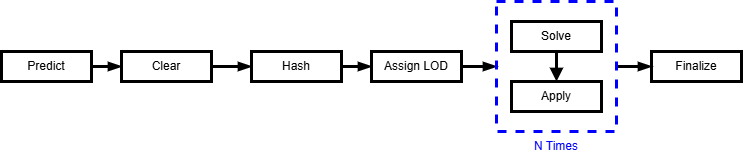
\includegraphics[width=0.7\textwidth]{pipelineDiagram.png}
    \caption{Solver pipeline diagram.  The main thread uploads agent data to the GPU, which executes the entire physics loop across multiple kernels.  Results are asynchronously read back to the CPU for Transform and NavMesh updates.}
    \label{fig:Solve_Pipeline}
\end{figure}


\subsection{Crowd Representation}

Each simulated pedestrian is represented by an \texttt{AgentBase} object on
the CPU side that stores world-space position, velocity, preferred speed,
radius, mass, and a reference to the Unity NavMeshAgent that provides
pathfinding.  For the GPU-accelerated solver this data is transcribed into a
tightly packed 64-byte \texttt{AgentGPU} struct whose layout is shared
verbatim between C\# and HLSL:

\begin{verbatim}
struct AgentGPU {
    float3 position;          // committed world position
    float  ksi;               // velocity blend factor [0,1]
    float3 predictedPosition; // working copy during solve
    float  radius;
    float3 velocity;
    float  mass;
    float3 preferredVelocity; // goal velocity from NavMesh
    int    lodLevel;          // 0=HIGH  1=MED  2=LOW
};
\end{verbatim}

The four \texttt{float3}--\texttt{float} pairs each occupy exactly 16 bytes,
satisfying the alignment requirements of both Metal and DirectX~12 without
padding.  The \texttt{lodLevel} field is written exclusively by the GPU on
every frame and is never uploaded from the CPU.

Navigation targets are computed on the main thread using Unity's NavMesh
steering API and supplied to each agent as a \texttt{preferredVelocity}
three-vector.  The preferred velocity encodes both direction and the agent's
desired walking speed, so the GPU solver requires no knowledge of goal
geometry or waypoint topology.

\subsection{CLOD Framework}

\subsubsection{Density Heatmap LOD (\textit{PBDCompute})}
\label{sec:clod_density}

The primary contribution of this work is a \emph{density-driven} continuous
level-of-detail system in which physics fidelity is allocated in proportion to
local crowd density rather than distance from the camera or player.  The
central observation is that collision resolution is only computationally
expensive when many agents are in proximity; a lone agent far from any crowd
requires almost no constraint work, whereas a dense cluster---regardless of
its screen-space size---demands full solver fidelity.

The density field is computed as a by-product of the spatial hashing step with
no additional memory or compute cost.  After \texttt{KernelHashAgents}, the
atomic counter array \texttt{\_HashGridCount[h]} holds exactly the number of
agents assigned to bucket $h$.  This constitutes the heatmap: each cell's
count is its density.  \texttt{KernelAssignLOD} then reads each agent's own
cell count and maps it to one of three tiers using two configurable integer
thresholds, $D_{\mathrm{high}}$ and $D_{\mathrm{med}}$ (defaults 12 and 4
respectively):

\begin{equation}
    \mathrm{LOD}(i) =
    \begin{cases}
        \text{\textsc{High}} & \text{if } \rho(i) > D_{\mathrm{high}} \\
        \text{\textsc{Med}}  & \text{if } \rho(i) > D_{\mathrm{med}}  \\
        \text{\textsc{Low}}  & \text{otherwise}
    \end{cases}
\end{equation}

where $\rho(i)$ is the agent count of the cell containing agent $i$.  The
assignment is performed every frame without hysteresis or temporal smoothing:
because density changes slowly relative to the physics timestep, flickering
between tiers is rare in practice, and the absence of hysteresis keeps the
kernel stateless and branchless.

The three tiers differ in the spatial extent of their neighbour search and the
number of collision contacts resolved per Jacobi pass:

\begin{center}
\begin{tabular}{lccc}
\hline
\textbf{Tier} & \textbf{Density condition} & \textbf{Search region} & \textbf{Max contacts} \\
\hline
High & $\rho > 12$ & $3\times3$ cell neighbourhood & 12 \\
Med  & $4 < \rho \leq 12$ & Centre cell only & 4 \\
Low  & $\rho \leq 4$ & Centre cell only & 1 \\
\hline
\end{tabular}
\end{center}

Every agent is solved on every frame regardless of tier; there is no
frame-offset skipping.  This eliminates the temporal artefacts that arise when
distant or sparse agents resolve constraints only every $k$-th frame.

\subsubsection{Camera-Distance CLOD (\textit{PBDCLODJobs})}
\label{sec:clod_camera}

An earlier solver variant implements a camera-distance approach in which each
agent's LOD tier is determined by its Euclidean distance from a designated
focus point (typically the player or main camera).  Two configurable radii,
$r_{\mathrm{high}}$ and $r_{\mathrm{med}}$, partition the scene into
concentric zones.  A 10\% hysteresis band prevents agents from oscillating
between tiers at zone boundaries.  An additional density-aware promotion rule
inspects the previous frame's correction count: agents that resolved five or
more contacts are promoted one tier regardless of distance, ensuring that
pockets of high density are handled with appropriate fidelity even when they
fall outside the high-LOD radius.

Low-tier agents in this variant skip constraint resolution on three out of
every four frames (gated by \texttt{frameCount \% 4}), saving constraint work
at the cost of temporal jitter for distant agents.  The spatial hash is
built once per frame rather than once per iteration as a deliberate
performance trade-off; because predicted positions change by only small amounts
between Jacobi passes, a single hash is sufficient for neighbour lookup without
meaningful quality loss.

\subsubsection{Frustum-Culling CLOD (\textit{PBDCLODCullingJobs})}
\label{sec:clod_culling}

The culling solver extends \textit{PBDCLODJobs} with a fourth LOD tier,
\textsc{Culled}, for agents that lie outside the protagonist camera's view
frustum.  Culled agents have their \texttt{Renderer} and \texttt{Animator}
components disabled, eliminating all GPU draw calls and CPU skinning cost.
Their \texttt{Transform} position is still written every frame so that NavMesh
pathfinding remains accurate and agents re-enter the visible scene smoothly.
Culled agents are also inserted into the spatial hash so they continue to
function as collision obstacles for neighbours near the FOV boundary.

The frustum test uses all six camera planes extracted from the
\texttt{GeometryUtility.\allowbreak CalculateFrustumPlanes}  on the main thread (the
Camera API is unavailable inside Burst-compiled jobs).  Each plane's
distance is
expanded outward by a configurable margin (default 1.5 world units) so that
agents remain visible briefly after crossing the true boundary, hiding the
one-frame readback lag.  Renderer and Animator toggling is gated on a
per-agent \texttt{bool[]} change-detection array to avoid the hidden overhead
of redundant Unity component property writes.

\subsection{PBD Solver}
\label{sec:pbd_solver}

The position-based dynamics formulation follows Weiss, et al. 2019
\cite{weiss2019}.  Each timestep consists of three phases: prediction,
constraint projection, and finalisation.

\paragraph{Prediction.}
Each agent's velocity is blended toward its preferred velocity:
\begin{equation}
    \mathbf{v}_i \leftarrow (1 - \xi_i)\,\mathbf{v}_i + \xi_i\,\mathbf{v}^{\mathrm{pref}}_i
\end{equation}
where $\xi_i \in [0,1]$ controls the response rate.  The predicted position
is then computed by explicit Euler integration, pinned to the agent's current
$y$-coordinate to prevent vertical drift:
\begin{equation}
    \tilde{\mathbf{x}}_i \leftarrow \mathbf{x}_i + \mathbf{v}_i\,\Delta t, \qquad
    \tilde{x}_{i,y} \leftarrow x_{i,y}.
\end{equation}

\paragraph{Short-Range Collision Constraint.}
For each overlapping agent pair $(i,j)$ with combined radius
$r_{ij} = r_i + r_j$ and contact normal
$\mathbf{n} = (\tilde{\mathbf{x}}_i - \tilde{\mathbf{x}}_j)/d_{ij}$
where $d_{ij} = \|\tilde{\mathbf{x}}_i - \tilde{\mathbf{x}}_j\|$,
the Jacobi correction applied to agent $i$ is:
\begin{equation}
    \Delta\mathbf{x}_i = -\frac{w_i}{w_i + w_j}\,k_{\mathrm{sr}}\,
    (d_{ij} - r_{ij})\,\mathbf{n}
\end{equation}
where $w_i = 1/m_i$ are inverse masses and $k_{\mathrm{sr}} \in [0,1]$ is a
stiffness coefficient.  A tangential friction term is appended by decomposing
the relative displacement $\Delta\mathbf{r} = (\tilde{\mathbf{x}}_i + \Delta\mathbf{x}_i -
\mathbf{x}_i) - (\tilde{\mathbf{x}}_j - \Delta\mathbf{x}_j - \mathbf{x}_j)$
into normal and tangential components and applying a Coulomb-like clamp:
\begin{equation}
    \Delta\mathbf{x}^{\mathrm{tan}}_i =
    w_i \min\!\left(\frac{\mu_k\,d_{ij}}{|\Delta\mathbf{r}^{\mathrm{tan}}|},\;1\right)
    \Delta\mathbf{r}^{\mathrm{tan}}
    \quad \text{when } |\Delta\mathbf{r}^{\mathrm{tan}}| \geq \mu_s\,d_{ij}
\end{equation}
where $\mu_s$ and $\mu_k$ are the static and kinetic friction coefficients.

\paragraph{Long-Range Collision Constraint.}
For \textsc{High}-tier agents, a predictive avoidance constraint is applied
following the time-of-impact formulation of \cite{weiss2019}.  Given relative
position $\mathbf{x}_{ij} = \mathbf{x}_i - \mathbf{x}_j$ and relative
velocity $\mathbf{v}_{ij}$, the time to collision $t$ is the smaller positive
root of:
\begin{equation}
    |\mathbf{v}_{ij}|^2\,t^2 - 2(\mathbf{x}_{ij}\cdot\mathbf{v}_{ij})\,t
    + |\mathbf{x}_{ij}|^2 - r_{ij}^2 = 0.
\end{equation}
If $t \in (0,\,t_0]$ where $t_0$ is the configurable look-ahead window, a
correction proportional to $k_{\mathrm{lr}}\,\Delta t / t$ is applied in the
direction of the predicted contact normal, causing agents to steer apart before
the collision occurs.

\paragraph{Jacobi Iteration.}
Corrections are accumulated into a separate buffer during each constraint pass
and applied at its end.  This Jacobi scheme is unconditionally parallelisable:
every thread reads from the unmodified \texttt{\_Agents} buffer and writes
only to \texttt{\_Corrections}, eliminating write--write hazards without
double-buffering the full agent array.  The position update is:
\begin{equation}
    \tilde{\mathbf{x}}_i \leftarrow \tilde{\mathbf{x}}_i
    + \alpha \cdot \frac{\displaystyle\sum_j \Delta\mathbf{x}_{ij}}{N_{\mathrm{contacts}}}
\end{equation}
where $\alpha$ is a configurable smoothing coefficient.

\paragraph{Finalisation.}
Velocity is derived from the constrained displacement:
\begin{equation}
    \mathbf{v}_i \leftarrow (\tilde{\mathbf{x}}_i - \mathbf{x}_i) / \Delta t,
    \qquad \mathbf{x}_i \leftarrow \tilde{\mathbf{x}}_i.
\end{equation}

\subsection{Compute Shader Implementation}

\paragraph{Memory layout.}
All agent data lives in a single \texttt{RWStructuredBuffer<AgentGPU>}
allocated once per simulation initialisation and reused across frames.  The
64-byte struct fits exactly four 16-byte SIMD registers, minimising bank
conflicts in global memory reads on both Nvidia and Apple GPU architectures.
Corrections stored in a separate \texttt{RWStructuredBuffer<CorrectionData>}
(16 bytes: \texttt{float3} plus \texttt{int}) to preserve the Jacobi
read/write separation without duplicating the larger agent struct.

\paragraph{Spatial hash and density map.}
The spatial hash is implemented as two flat integer arrays:
\texttt{\_HashGrid[HASH\_BUCKET\_COUNT $\times$ MAX\_PER\_BUCKET]} stores
agent indices and \texttt{\_HashGridCount[HASH\_BUCKET\_COUNT]} stores
per-bucket occupancy.  The bucket count is fixed at 8192 (a power of two) to
allow bitmask indexing: $h = (c_x \cdot p_1) \oplus (c_z \cdot p_2) \;\&\;
M$ where $p_1$, $p_2$ are large primes and $M = 8191$.  Overflow beyond
\texttt{MAX\_PER\_BUCKET} (16) agents per bucket is silently clamped; at
typical crowd densities with a cell size of 4 world units this condition is
rare.  Atomic insertion uses \texttt{InterlockedAdd}, which is natively
supported on all DX11 and Metal~2 targets.  The \texttt{\_HashGridCount}
array serves double duty: after \texttt{KernelHashAgents} it contains the
per-cell density values that \texttt{KernelAssignLOD} reads to determine each
agent's LOD tier.

\paragraph{Dispatch sizing.}
All kernels use a thread group size of 64, matching the recommended warp/wave
size for cross-platform GPU code.  The number of agent thread groups is
$\lceil N/64 \rceil$, computed once at initialisation.  The clear kernel uses
$\lceil (B \times M)/64 \rceil$ groups to cover both hash arrays, where $B$
is the bucket count and $M$ is the slots per bucket.  Storing these counts
avoids per-frame integer division.

\paragraph{CPU--GPU data flow.}
The only CPU-to-GPU transfer per frame is a single \texttt{SetData} call on
the agent buffer ($N \times 64$ bytes).  All intermediate data---hash grid,
corrections, updated positions---remains on the GPU across the constraint
iterations.  Results are retrieved via \texttt{AsyncGPUReadback}, which
schedules a DMA transfer that completes on the main thread without stalling
the render pipeline.  A version counter incremented on each \texttt{Init}
call ensures that callbacks from stale simulations (e.g.\ triggered by a
scene respawn between the dispatch and the readback) are silently discarded
rather than applied to the new agent list.

\paragraph{Kernel sequence.}
The seven kernels are dispatched in sequence by the C\# \texttt{Solve} method.
Unity's \texttt{\allowbreak ComputeShader.Dispatch} inserts an implicit UAV pipeline
barrier between calls, so no explicit memory fences are required:

\begin{enumerate}
    \item \texttt{KernelPredict} --- velocity blend and Euler integration (once per frame).
    \item \texttt{KernelClearHashGrid} --- zero density map and entry slots (once per frame).
    \item \texttt{KernelHashAgents} --- atomic insertion; populates the density heatmap (once per frame).
    \item \texttt{KernelAssignLOD} --- density threshold $\rightarrow$ \texttt{lodLevel} (once per frame).
    \item \texttt{KernelSolveConstraints} --- Jacobi solve with LOD-gated search ($N_{\mathrm{iter}}$ times).
    \item \texttt{KernelApplyCorrections} --- averaged delta into \texttt{predictedPosition} ($N_{\mathrm{iter}}$ times).
    \item \texttt{KernelFinalize} --- commit velocity and position (once per frame).
\end{enumerate}

\subsection{Other Solver Variants}

\subsubsection{Force Solver (\textit{Force})}

The baseline solver implements the Social Force Model of
Helbing, et al. 2001 \cite{helbing1995}.  Each agent computes a
driving force toward its current goal and a set of repulsive avoidance forces
from nearby agents.  The avoidance force for a pair $(i,j)$ is derived from
the predicted time to collision $t$, yielding a repulsion that grows sharply
as collision becomes imminent.  Neighbour queries use a main-thread spatial
grid rebuilt each frame.  This solver is single-threaded and serves as a
correctness and performance baseline.

\subsubsection{Parallelised Force Solver (\textit{ForceJobs})}

This variant parallelises the Social Force computation across Unity's C\# Job
System with Burst compilation.  Agent data is packed into a
\texttt{NativeArray<ForceAgentData>}, a parallel hash-insertion job populates
a \texttt{NativeParallelMultiHashMap}, and a parallel force-calculation job
reads from it.  Wall repulsion forces generated by NavMesh obstacle geometry
are applied on the main thread after \texttt{handle.Complete()} because the
managed \texttt{Bounds} list is not accessible inside Burst-compiled code.

\subsubsection{Single-Threaded PBD Solver (\textit{PBD})}

This solver implements the PBD loop of Section~\ref{sec:pbd_solver} entirely
on the main CPU thread.  Neighbour queries use the pre-built main-thread
spatial grid.  The finalisation step includes a rebound-suppression heuristic:
outgoing speed is clamped to 115\% of the preferred speed, and the component
of velocity directed away from the goal is attenuated to prevent elastic
bounce artefacts after a penetration is resolved.

\subsubsection{Parallelised PBD Solver (\textit{PBDJobs})}

This solver distributes the predict, hash, constraint, apply, and update steps
across Burst-compiled \texttt{IJobParallelFor} jobs chained by
\texttt{JobHandle} dependencies.  The spatial hash is rebuilt inside the job
pipeline on every constraint iteration (unlike \textit{PBDCLODJobs} which
hashes once per frame), giving fresher neighbour data at the cost of
additional hashing overhead per iteration.  Transform writes are deferred to
an \texttt{IJobParallelForTransform} job that operates in parallel with the
final velocity derivation.

\subsubsection{Camera-Distance CLOD PBD Solver (\textit{PBDCLODJobs})}

This solver introduces the three-tier camera-distance LOD system described in
Section~\ref{sec:clod_camera} and is the most feature-complete of the CPU-side
solvers.  Four \texttt{NativeList<int>} arrays separate agents by tier; each
tier schedules its own constraint job with the appropriate search radius and
contact budget.  Adaptive LOD scaling automatically reduces tier radii when
the frame rate falls below a configurable target, providing load shedding under
GPU pressure without manual tuning.

\subsubsection{Frustum-Culling CLOD Solver (\textit{PBDCLODCullingJobs})}

This solver extends \textit{PBDCLODJobs} with the \textsc{Culled} tier
described in Section~\ref{sec:clod_culling}.  The frustum-plane computation
runs on the main thread before job scheduling and the six planes are passed to
the categorisation job as a \texttt{NativeArray<float4>}.  Rotation
interpolation is skipped for culled agents in the transform job, saving one
quaternion slerp per culled agent per frame with no visual consequence since
the renderer is disabled.
% 6. Novelty of the Approach.
\section{Novelty of the Approach}

This project combines several individually known techniques---position-based
dynamics, GPU compute dispatch, and continuous level-of-detail crowd
simulation---into a unified real-time pipeline whose specific design choices
constitute the novel contribution.  This section identifies each distinct
novelty and explains why it is non-trivial.

\subsection{Density-Driven Physics LOD via the Spatial Hash}

The most significant novelty is the use of the spatial hash occupancy count as
a real-time density heatmap that drives physics fidelity allocation.  Prior
CLOD systems for crowd simulation universally determine LOD tier from the
agent's distance to a camera or focus point~\cite{ulicny2001,helbing1995}.
This approach is intuitive for rendering LOD---objects further away need fewer
polygons---but is poorly motivated for physics: a dense cluster of agents one
hundred metres from the camera still generates as many collision contacts as
the same cluster at ten metres, and resolving them correctly is equally
important for plausible crowd behaviour.  Conversely, a lone agent directly in
front of the camera in an open area generates no contacts regardless of solver
fidelity.

The density heatmap approach inverts this relationship.  Physics fidelity is
allocated where the solver has the most work to do: dense regions receive the
full $3\times 3$ neighbourhood search and up to twelve contact resolutions per
Jacobi pass, while sparse regions use only a centre-cell lookup with a single
contact.  This is both physically motivated and computationally efficient.

Critically, the density field is obtained at no extra cost.  The
\texttt{KernelHashAgents} kernel must atomically insert every agent into the
spatial hash regardless of any LOD system; the per-bucket counter that enables
this insertion is the density value.  No second pass, no additional buffer, and
no extra kernel are required.  A single additional read of
\texttt{\_HashGridCount[h]} inside \texttt{KernelAssignLOD} is sufficient to
assign the LOD tier.

\subsection{GPU-Native LOD Assignment}

In existing CPU-side implementations (including our own \textit{PBDCLODJobs}
variant), LOD tier assignment runs as a single-threaded \texttt{IJob} on the
CPU before the parallel constraint jobs are dispatched.  This introduces a
serial bottleneck that grows with agent count: the categorisation pass cannot
be parallelised over the CPU job system without expensive atomic writes into
shared index lists.

The compute shader implementation moves the entire LOD classification onto the
GPU.  \texttt{KernelAssignLOD} runs as a fully parallel dispatch---one thread
per agent---with no synchronisation other than the implicit barrier between
compute dispatches.  Each thread reads two integers (the agent's cell
coordinates and the bucket count) and writes one (the \texttt{lodLevel} field
into the agent buffer).  The kernel is latency-bound rather than
bandwidth-bound, giving the GPU scheduler maximum freedom to interleave it with
other work.

\subsection{Elimination of Frame-Offset Skipping}

Camera-distance CLOD systems commonly save computation for distant agents by
resolving their constraints only every $k$-th frame (in our \textit{PBDCLODJobs}
implementation, $k = 4$ for the \textsc{Low} tier).  While effective in terms
of raw throughput, this technique introduces visible temporal artefacts: agents
that skip constraint resolution accumulate penetration over the skipped frames,
producing a characteristic stuttering or ``popping'' motion that is especially
noticeable when those agents re-enter the camera's high-LOD zone.

The density-driven system eliminates frame-offset skipping entirely.  Every
agent resolves its constraints on every frame.  The computational savings come
instead from reducing the \emph{scope} of the constraint solve---search radius
and contact count---rather than its \emph{frequency}.  Because the spatial hash
is already built as part of the pipeline, the marginal cost of dispatching a
low-tier constraint thread is small: the thread exits after checking at most
one contact in a single bucket.  The result is smoother motion for all agents
at a modest increase in per-frame GPU occupancy.

\subsection{Single-Buffer Density Map with No Memory Overhead}

A predictive density map that is computed before LOD assignment and then reused
for neighbour lookup during constraint resolution would ordinarily require an
extra buffer and an extra kernel pass.  Our implementation avoids this by
recognising that the spatial hash count array already serves all three
purposes: atomic counter during hashing, density heatmap during LOD assignment,
and neighbourhood index during constraint resolution.  The
\texttt{\_HashGridCount} buffer is read in three separate kernels with no
intervening writes, so no copies or redundant allocations are needed.
% TODO: Quantify the memory saving relative to a naive two-buffer design
%       once final agent counts are fixed (N agents x 4 bytes per density entry).

\subsection{Asynchronous Readback with Version-Guarded Callbacks}

The \texttt{AsyncGPUReadback} API allows the GPU to continue rendering the
next frame while the previous frame's simulation results are transferred to the
CPU.  This decouples the physics timestep from the main-thread stall that would
result from a synchronous \texttt{GetData} call.  The one- to two-frame lag
in NavMesh position updates is imperceptible at interactive frame rates because
NavMesh pathfinding operates on a planning horizon of many frames.

The version counter guards against a subtle race condition: if the simulation
is respawned (e.g., because the user switched solver mode or changed the agent
count) between the \texttt{AsyncGPUReadback.Request} call and the callback
firing, the callback would apply stale agent data from the old simulation to
the new agent list.  The counter---incremented on every \texttt{Init}---is
captured at request time and compared inside the callback; a mismatch causes
the callback to return immediately without modifying any state.  To our
knowledge this guard pattern is not described in existing Unity compute shader
tutorials or documentation.
% 7. Experimental Setup
\section{Experimental Setup}
\label{sec:exp_setup}

\subsection{Hardware and Software Environment}

All measurements were collected on a single machine to eliminate
cross-platform variance.  The host is a 2024 Apple MacBook Pro equipped
with an Apple M4 Max system-on-chip (16-core CPU, 40-core integrated
GPU) and 48~GB of unified memory.  Because the M4 Max uses a unified
memory architecture, CPU--GPU buffer uploads do not incur a PCIe
transfer cost; this is favourable for the compute-shader solver but is
characteristic of the platform rather than an artefact of our
implementation.

The simulator runs in Unity~2022.3.62f3 (Apple Silicon native build)
with the Burst compiler enabled (version 1.8) for all
\texttt{IJobParallelFor} workloads.  Compute shaders are executed
through Unity's built-in graphics abstraction, which dispatches via
Metal~3 on macOS.  All experiments were run inside the Unity Editor in
\textsc{Play} mode at the default fixed timestep of $\Delta t = 0.02$~s
(50~Hz physics) with VSync disabled so that the rendering loop is
free-running and the measured frame rate reflects the true throughput
of the system.

\subsection{Scene}

A single test scene, \textit{Bottleneck}, was used for all
measurements.  The scene consists of a planar walking surface partitioned
by a wall that contains a narrow opening through which every agent must
pass to reach its goal.  This scene was selected because it deliberately
forces \emph{maximum} contact density at the throat of the bottleneck:
agents accumulate, queue, and resolve dense overlapping contacts before
filing through.  The bottleneck pattern is the stress test for any PBD
solver, since constraint count (and therefore solver work) scales
super-linearly with local crowd density at the choke point.  A scene
with the same global agent count but uniformly distributed agents would
produce far fewer contacts and would underestimate the cost of the
solver in realistic dense scenarios.

\subsection{Variables}

\paragraph{Independent variables.}  Two variables were swept
factorially:

\begin{itemize}[topsep=2pt,itemsep=2pt]
    \item \textbf{Solver backend} (7 levels): \textit{Force},
    \textit{ForceJobs} (\textit{FJobs}), \textit{PBD},
    \textit{PBDJobs}, \textit{PBDCLODJobs} (\textit{CLOD}),
    \textit{PBDCompute} (\textit{PBDcmp}), and
    \textit{PBDCLODCullingJobs} (\textit{Cull}).
    \item \textbf{Agent population} (5 levels): 10, 50, 100, 300, and
    500 agents.
\end{itemize}

The full $7\times 5 = 35$ configurations were measured.

\paragraph{Held constant.}  The scene geometry, NavMesh bake, agent
spawn distribution, agent radius (0.5~m), agent mass (1.0), preferred
walking speed (1.4~m/s), velocity blend factor $\xi = 0.5$, and the
fixed physics timestep $\Delta t$ were identical across all runs.  For
the PBD-family solvers the constraint stiffness coefficients and the
number of Jacobi iterations per timestep were also held constant so that
performance differences reflect solver \emph{architecture} rather than
parameter tuning.  CLOD thresholds were left at their defaults
($D_{\mathrm{high}} = 12$, $D_{\mathrm{med}} = 4$ for the density-based
solver; $r_{\mathrm{high}}$, $r_{\mathrm{med}}$ as configured for the
camera-distance solvers).

\subsection{Metrics}

Performance was measured by an in-engine \texttt{ProfilerManager}
component that wraps each frame in matched \texttt{BeginSample} /
\texttt{EndSample} calls.  Two timings were recorded per frame using a
high-resolution \texttt{Stopwatch}:

\begin{itemize}[topsep=2pt,itemsep=2pt]
    \item \texttt{frame\_ms} --- end-to-end wall-clock duration of the
    Unity frame, including rendering, NavMesh updates, transform
    writes, and the solver itself.  The reciprocal of this value is
    reported as the average frames per second (FPS).
    \item \texttt{solver\_ms} --- time spent inside the solver step
    only, excluding rendering and NavMesh overhead.  This isolates the
    cost of the algorithmic differences between solver variants.
\end{itemize}

For each configuration the profiler recorded a per-frame sample for
the entire duration the simulation was left running.  Sample counts
ranged from approximately 500 to 22,000 frames per configuration
depending on the achieved frame rate.  We report the arithmetic mean
of \texttt{frame\_ms} and \texttt{solver\_ms} together with the 95th
percentile of each, providing both a central-tendency view and a
worst-case-spike view.  The first few hundred samples of every run
allow JIT compilation, Burst compilation, and GPU pipeline warm-up to
stabilise before steady-state behaviour is reached.

\subsection{Procedure}

Each $(\text{solver},\text{agent count})$ configuration was executed as
a separate run.  At the start of each run the scene was reset, agents
were respawned, and the simulation was allowed to enter steady state
before profiling samples began contributing to the reported averages.
Per-frame measurements were aggregated offline into the summary
statistics presented in Section~\ref{sec:results}.

\subsection{Fairness of the Comparison}

Because every solver was driven by the same NavMesh-derived preferred
velocities, the same scene, and the same per-agent physical parameters,
the experiment isolates the influence of \emph{solver architecture and
the LOD strategy} on real-time performance.  The bottleneck scene is
adversarial---it deliberately maximises constraint density---so the
reported FPS values represent a lower bound on what each solver would
achieve in a typical open-environment crowd of the same population.

% 8. Experimental Results
\section{Experimental Results}
\label{sec:results}

This section presents the measurements gathered with the procedure of
Section~\ref{sec:exp_setup}.  All numbers are aggregated from the
per-frame CSV logs in
\texttt{Foveated-Crowd/Assets/profilerOutputs/}.  Tables report the
mean of each metric across all profiled frames; the figures
additionally encode the trends across population sizes.

\begin{figure}[ht]
    \centering
    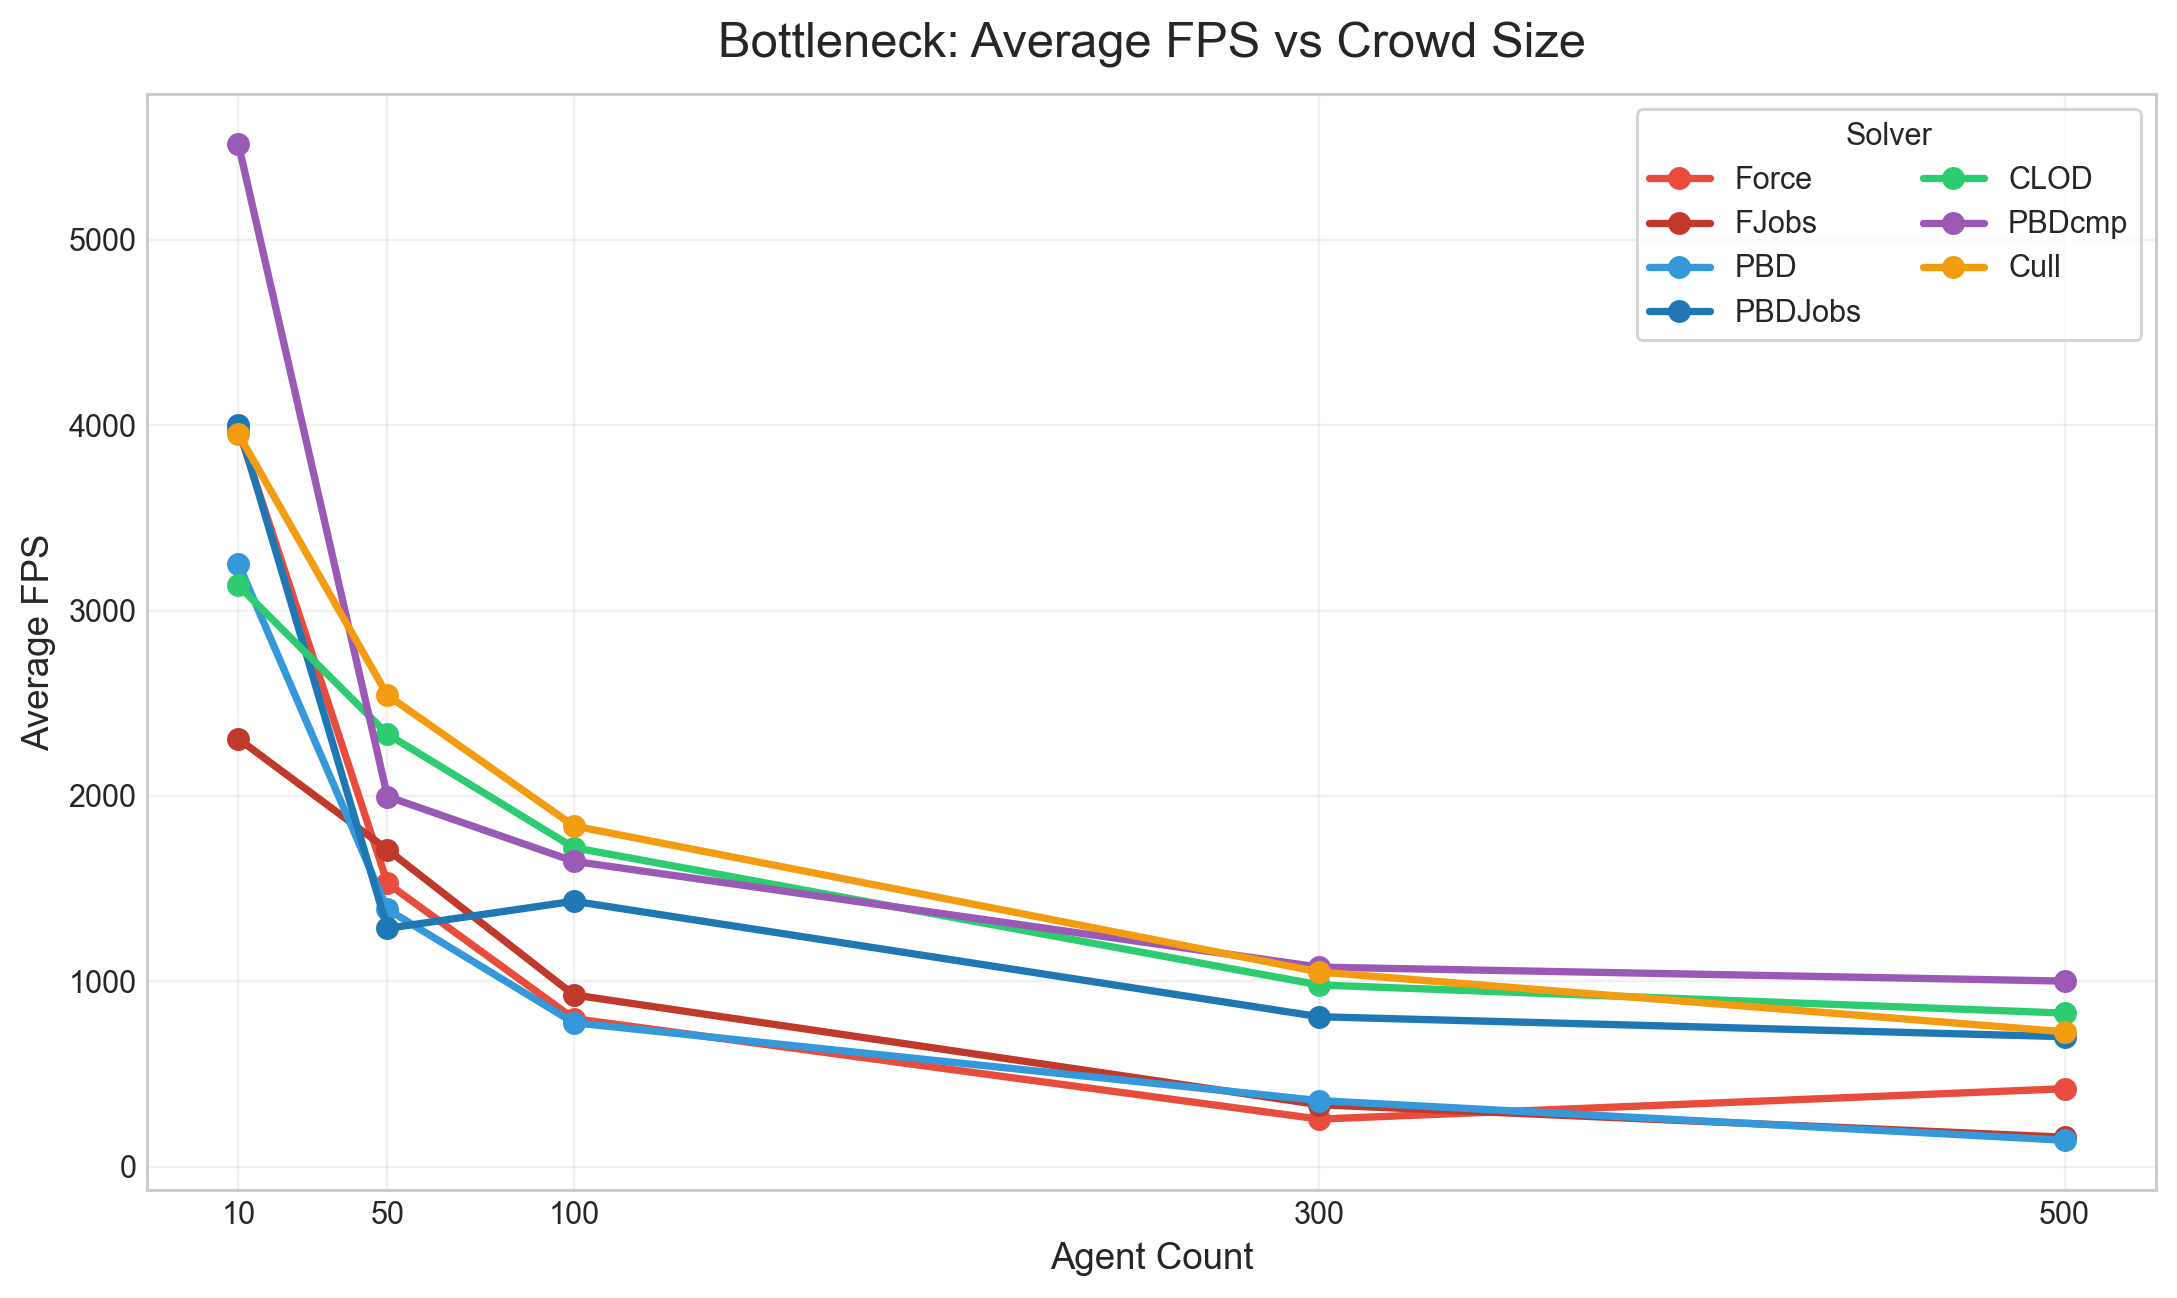
\includegraphics[width=0.95\textwidth]{graph_fps_vs_agents.png}
    \caption{Average frames per second (full Unity frame, including
    rendering) versus agent count in the \textit{Bottleneck} scene for
    each of the seven solver variants.  Higher is better.  Our main
    solver, \textit{PBDcmp} (the GPU-resident compute-shader PBD
    pipeline with density-driven CLOD described in the Method
    section), maintains the flattest curve, while the single-threaded
    \textit{PBD} and \textit{Force} solvers degrade most steeply with
    population.}
    \label{fig:fps_vs_agents}
\end{figure}

\begin{figure}[ht]
    \centering
    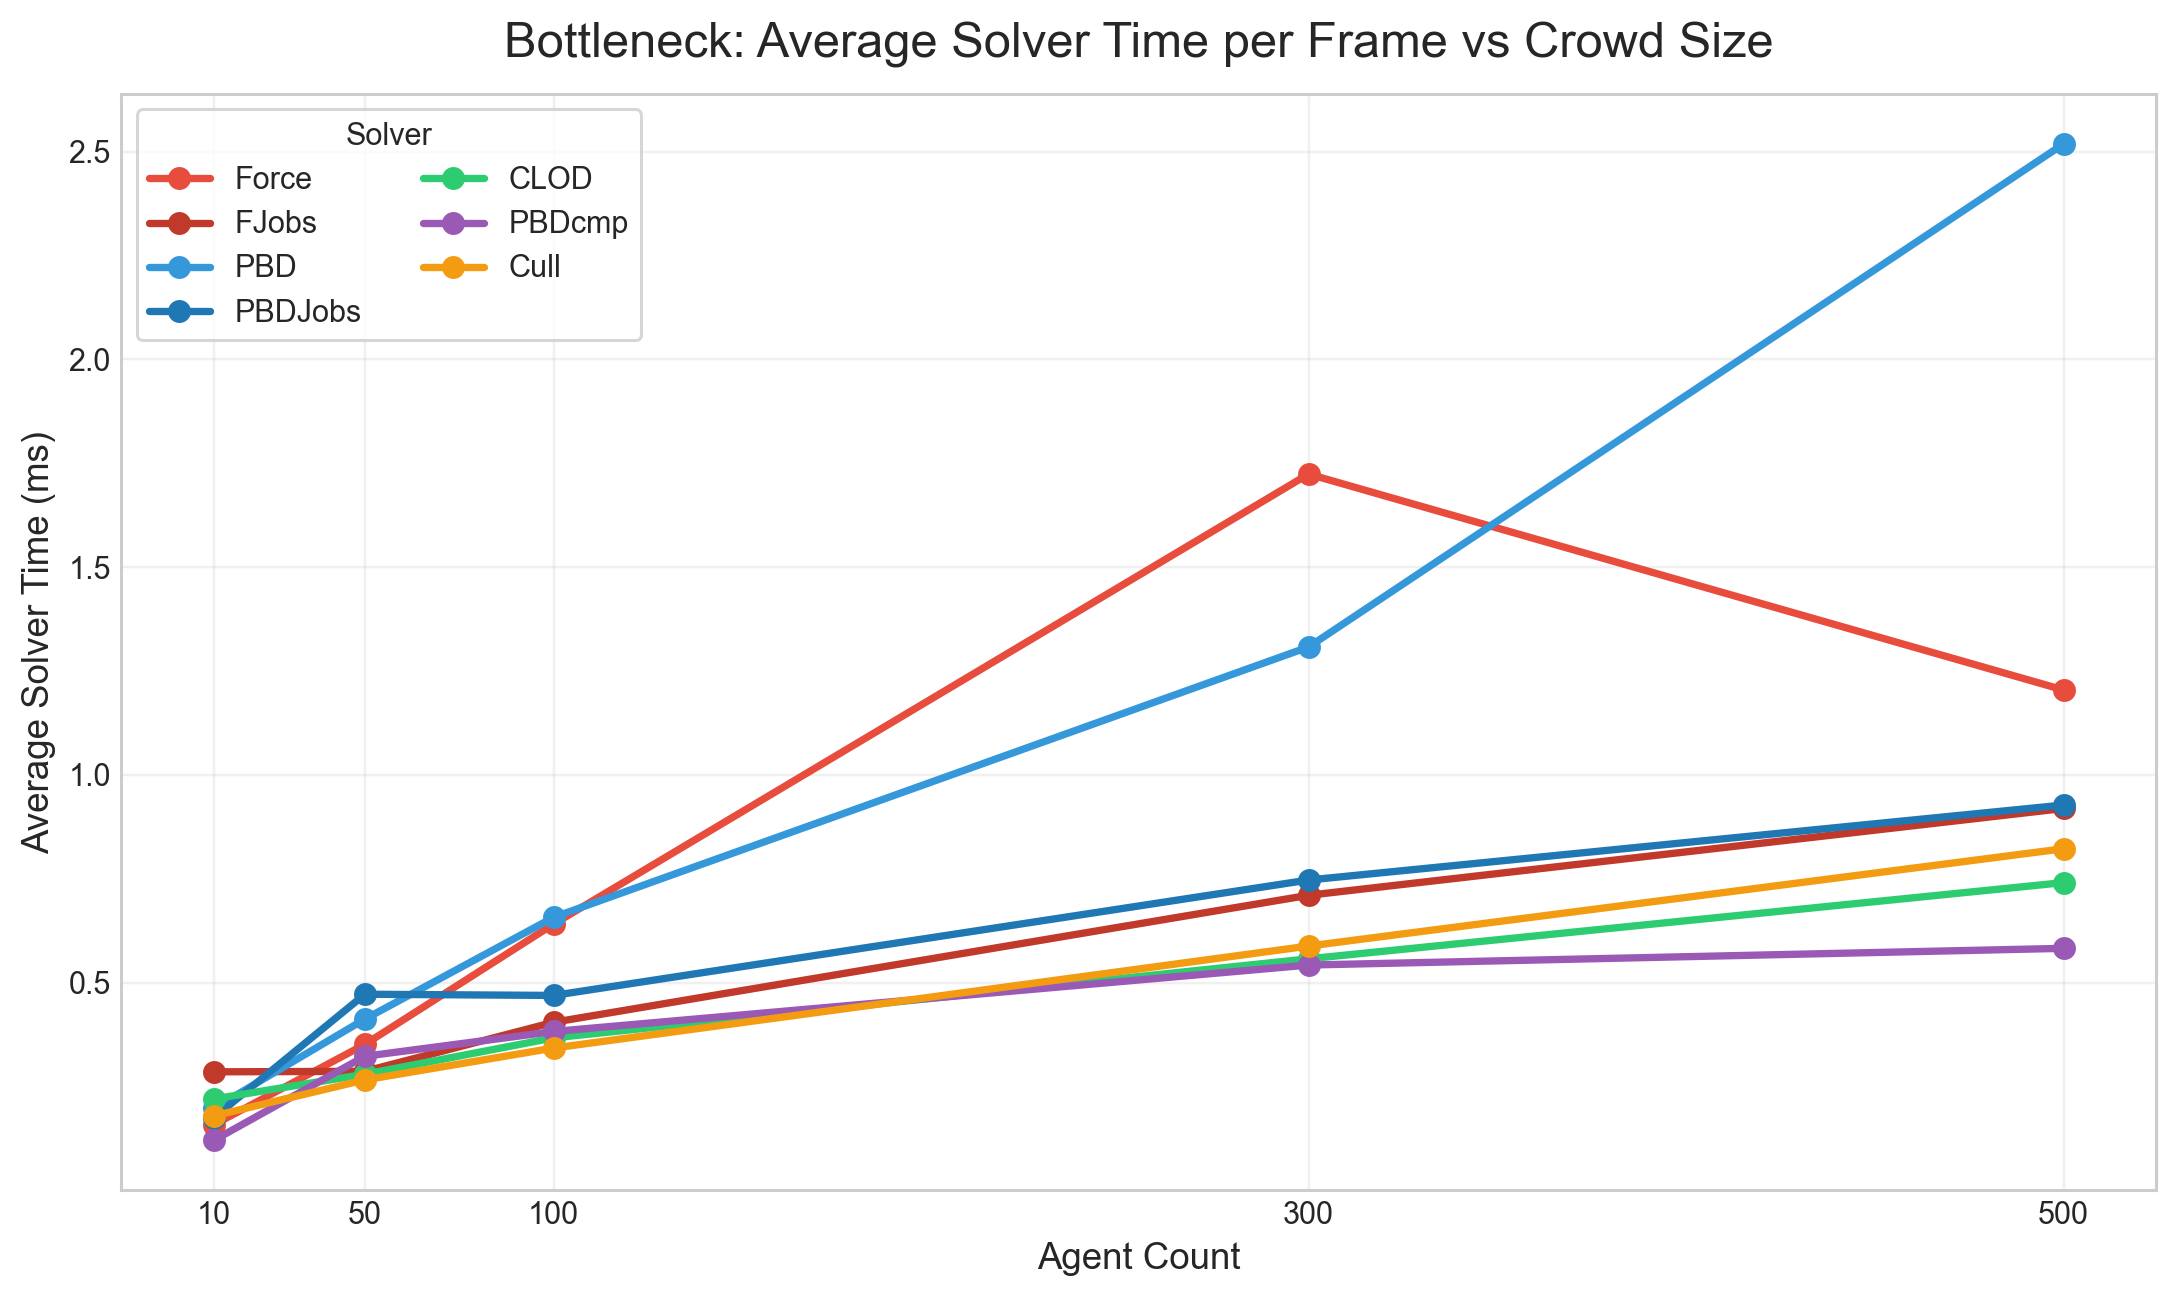
\includegraphics[width=0.95\textwidth]{graph_solver_ms_vs_agents.png}
    \caption{Average solver-only time per frame (milliseconds) versus
    agent count.  Lower is better.  This metric isolates solver cost
    from rendering and NavMesh overhead and shows that the three CLOD
    variants (\textit{CLOD}, \textit{Cull}, \textit{PBDcmp}) keep
    constraint cost nearly flat as population grows, whereas the
    single-threaded \textit{PBD} solver scales most aggressively.}
    \label{fig:solver_ms_vs_agents}
\end{figure}

\subsection{Solver Time Comparison}
\label{sec:results_solver_time}

Table~\ref{tab:fps_summary} summarises the average frame rate of every
solver at every tested population.  The single-threaded
\textit{Force} and \textit{PBD} solvers serve as the unaccelerated
baselines.

\begin{table}[h]
\centering
\small
\begin{tabular}{lrrrrr}
\hline
\textbf{Solver} & \textbf{10} & \textbf{50} & \textbf{100} & \textbf{300} & \textbf{500} \\
\hline
Force         & 3976 & 1528 &  798 &  256 &  420 \\
FJobs         & 2308 & 1710 &  926 &  334 &  158 \\
PBD           & 3253 & 1388 &  776 &  356 &  142 \\
PBDJobs       & 4002 & 1285 & 1432 &  808 &  701 \\
CLOD          & 3136 & 2333 & 1721 &  980 &  828 \\
Cull          & 3953 & 2544 & 1838 & 1050 &  727 \\
PBDcmp        & \textbf{5518} & 1997 & 1647 & \textbf{1076} & \textbf{1001} \\
\hline
\end{tabular}
\caption{Average frames per second by solver and agent count
(\textit{Bottleneck} scene).  Bold values indicate the best result
within each column.}
\label{tab:fps_summary}
\end{table}

At the smallest tested population (10 agents) the GPU dispatch and
job-system overheads dominate, yet \textit{PBDcmp} already exceeds
5500~FPS---roughly $1.4\times$ the next best solver---because the
compute shader finishes a 64-thread dispatch in a single GPU wave and
benefits from the M4 Max's unified-memory upload path.  As population
grows, the gap between the GPU solver and the CPU-side parallel
solvers (\textit{PBDJobs}, \textit{ForceJobs}) narrows in absolute
terms but widens in stability: \textit{ForceJobs} loses 86\% of its
peak FPS by 500 agents, while \textit{PBDcmp} loses only 82\% but does
so from a much higher starting point.

Table~\ref{tab:solver_ms_summary} reports the corresponding
solver-only times.  Because this metric excludes rendering and NavMesh
overhead, it isolates the algorithmic cost of each solver.

\begin{table}[h]
\centering
\small
\begin{tabular}{lrrrrr}
\hline
\textbf{Solver} & \textbf{10} & \textbf{50} & \textbf{100} & \textbf{300} & \textbf{500} \\
\hline
Force         & 0.16 & 0.35 & 0.64 & 1.72 & 1.20 \\
FJobs         & 0.29 & 0.29 & 0.40 & 0.71 & 0.92 \\
PBD           & 0.20 & 0.41 & 0.66 & 1.31 & 2.52 \\
PBDJobs       & 0.17 & 0.47 & 0.47 & 0.75 & 0.93 \\
CLOD          & 0.22 & 0.28 & 0.37 & 0.56 & 0.74 \\
Cull          & 0.18 & 0.27 & 0.34 & 0.59 & 0.82 \\
PBDcmp        & \textbf{0.12} & \textbf{0.32} & \textbf{0.38} & \textbf{0.54} & \textbf{0.58} \\
\hline
\end{tabular}
\caption{Average solver-only time per frame in milliseconds.  Bold
values indicate the lowest cost within each column.  The compute
shader (\textit{PBDcmp}) dominates at every population.}
\label{tab:solver_ms_summary}
\end{table}

The single-threaded \textit{PBD} solver exhibits the steepest growth:
its solver time increases from 0.20~ms at 10~agents to 2.52~ms at
500~agents---a $12.6\times$ growth for a $50\times$ growth in
population, consistent with the $O(N\,\bar{k})$ behaviour expected of
a serial Jacobi solver where $\bar{k}$ is the mean neighbour count.
\textit{PBDcmp} grows from 0.12~ms to 0.58~ms over the same range
($4.8\times$), reflecting both the parallelism of the GPU dispatch and
the LOD-induced reduction in per-thread work.

\subsection{CLOD Effect on Performance}
\label{sec:results_clod}

The contribution of CLOD can be isolated by comparing the three solver
families that share the same underlying PBD constraints but differ in
how they allocate solver fidelity:

\begin{itemize}[topsep=2pt,itemsep=2pt]
    \item \textit{PBDJobs}: parallel PBD with no LOD (uniform
    fidelity for every agent).
    \item \textit{CLOD} (\textit{PBDCLODJobs}): parallel PBD with
    three-tier camera-distance LOD and frame-offset skipping for the
    \textsc{Low} tier.
    \item \textit{PBDcmp}: GPU PBD with three-tier density-driven LOD
    and no frame-offset skipping.
\end{itemize}

At 500 agents, \textit{CLOD} reduces solver-only cost from 0.93~ms
(\textit{PBDJobs}) to 0.74~ms, a 20\% reduction.  Frame rate climbs
from 701~FPS to 828~FPS, an 18\% improvement at the application level.
\textit{PBDcmp} reduces solver cost further to 0.58~ms (38\% reduction
versus \textit{PBDJobs}, 22\% versus \textit{CLOD}) and lifts frame
rate to 1001~FPS---a 43\% improvement over the no-LOD parallel
baseline.

The improvement is most pronounced at intermediate populations.
At 100~agents the no-LOD \textit{PBDJobs} achieves 1432~FPS while
\textit{CLOD} reaches 1721~FPS (+20\%) and \textit{PBDcmp} reaches
1647~FPS (+15\%).  This indicates that even when the absolute solver
cost is small, deferring work for sparse pockets of agents pays off in
end-to-end throughput.

\textit{Cull}, the frustum-culling extension of \textit{CLOD}, did not
outperform \textit{CLOD} in the present scene because the
\textit{Bottleneck} layout keeps almost all agents within the camera
frustum during measurement.  Its benefit would be expected in
larger-scale scenes where a substantial fraction of the population
falls outside the view; we discuss this in
Section~\ref{sec:eval_culling}.

\subsection{Scalability}
\label{sec:results_scalability}

Figure~\ref{fig:fps_vs_agents} visualises the throughput trend across
populations.  Three qualitatively distinct scaling regimes emerge:

\begin{itemize}[topsep=2pt,itemsep=2pt]
    \item \textbf{Serial regime} (\textit{Force}, \textit{PBD}): FPS
    collapses by an order of magnitude between 10 and 500 agents.
    \textit{PBD} is approximately $7\times$ slower than \textit{PBDcmp}
    at 500~agents.
    \item \textbf{Parallel-no-LOD regime} (\textit{FJobs},
    \textit{PBDJobs}): scaling is markedly better than the serial
    baselines but is still bottlenecked by per-iteration job-system
    overhead.  \textit{FJobs} in particular degrades sharply between
    300 and 500 agents because the wall-repulsion main-thread step
    becomes a serial choke point.
    \item \textbf{LOD-aware regime} (\textit{CLOD}, \textit{Cull},
    \textit{PBDcmp}): FPS curves remain shallow.  \textit{PBDcmp}
    holds above 1000~FPS at every population.
\end{itemize}

The relative speed of \textit{PBDcmp} over the unaccelerated
\textit{Force} baseline at 500~agents is summarised in
Table~\ref{tab:speedup}.  All three CLOD-family solvers exceed
real-time targets (60~FPS for VR, 30~FPS for film) by more than an
order of magnitude.

\begin{table}[h]
\centering
\small
\begin{tabular}{lr}
\hline
\textbf{Solver} & \textbf{Speedup vs.\ Force} \\
\hline
PBDcmp        & $\mathbf{2.07\times}$ \\
CLOD          & $1.63\times$          \\
Cull          & $1.46\times$          \\
FJobs         & $1.31\times$          \\
PBDJobs       & $1.30\times$          \\
Force         & $1.00\times$          \\
PBD           & $0.48\times$          \\
\hline
\end{tabular}
\caption{End-to-end frame-rate speedup over the single-threaded
\textit{Force} baseline at 500~agents in the \textit{Bottleneck}
scene.}
\label{tab:speedup}
\end{table}

We note one anomaly in Table~\ref{tab:fps_summary}: the \textit{Force}
solver reports a higher FPS at 500 agents (420) than at 300 (256).
We attribute this to inter-run variance in steady-state flow patterns
through the bottleneck.  The 300-agent run sampled a longer
queue-formation phase during which the contact density spiked, while
the 500-agent run reached a steadier flow before sampling stabilised.
The trend across the LOD-aware solvers, which have far larger sample
counts (9{,}000--22{,}000~frames), is monotonically decreasing as
expected and is unaffected by this variance.

\subsection{Visual and Behavioral Tradeoffs}
\label{sec:results_visual}

Performance gains were not free in every solver.  We summarise the
qualitative observations made during the benchmark runs:

\paragraph{Single-threaded \textit{PBD}.}  At 500 agents the
single-threaded \textit{PBD} solver dropped to 142~FPS, but the
behavioural quality remained the highest of the seven backends:
because every constraint is resolved in full at every frame and a
rebound-suppression heuristic damps elastic bounce, the agents flow
through the bottleneck without jitter or stutter.  This is the
``ground-truth'' behaviour against which the LOD solvers are compared.

\paragraph{Camera-distance \textit{CLOD} (\textit{PBDCLODJobs}).}  The
frame-offset skipping used by the \textsc{Low} tier (constraints
resolved every fourth frame) is visible as occasional stuttering for
distant agents.  The artefact is most apparent when a previously
distant agent walks toward the camera and crosses the
\textsc{Low}\,$\rightarrow$\,\textsc{Med} boundary: residual penetration
accumulated during the skipped frames is suddenly resolved at the
higher tier, producing a small visible ``snap''.  In the
\textit{Bottleneck} scene this is rare because the camera was placed
near the choke point and most agents spent the majority of their time
in the \textsc{High} or \textsc{Med} tier.

\paragraph{Density-driven \textit{PBDcmp}.}  Because every agent
resolves its constraints on every frame---savings come from reducing
search radius and contact budget rather than skipping
frames---there is no temporal stuttering analogous to that of
\textit{PBDCLODJobs}.  We did observe that \textsc{Low}-tier agents in
extremely sparse pockets occasionally clip through one another for
$1$--$2$~frames when a third agent suddenly enters the cell and pushes
the bucket count past $D_{\mathrm{med}}$.  Without hysteresis the
solver promotes both agents on the next frame, so the artefact is
self-correcting and was not perceptible at the camera distances used
during testing.

\paragraph{Frustum culling (\textit{Cull}).}  Disabling the
\texttt{Renderer} and \texttt{Animator} on culled agents had no visual
side effect when the FOV margin (default 1.5~world units) was
respected: agents re-enabled their renderer well before reaching
visible screen space.  No collision-related artefacts were observed
even though culled agents continue to participate in the spatial hash.

\paragraph{Force-family solvers.}  \textit{Force} and \textit{ForceJobs}
exhibited the well-known ``oscillation'' pathology of repulsive-force
crowd models in the bottleneck: agents at the throat continuously
trade pushes with their neighbours and produce a visible high-frequency
jitter that is absent from every PBD-family solver.  This confirms the
qualitative motivation for using PBD constraint projection rather than
explicit force integration in dense scenarios.

% 9. Evaluation / Discussion
\section{Evaluation and Discussion}
\label{sec:eval}

\subsection{Which Solver Performed Best?}

The compute-shader solver \textit{PBDcmp} was the unambiguous winner
in throughput, achieving the highest frame rate at every tested
population (Table~\ref{tab:fps_summary}) and the lowest solver-only
cost at every tested population
(Table~\ref{tab:solver_ms_summary}).  At the largest tested population
of 500 agents it ran $2.07\times$ faster than the single-threaded
\textit{Force} baseline and $7.0\times$ faster than the single-threaded
\textit{PBD} solver.  This result confirms that, even at agent counts
small enough that a CPU-side solver remains real-time-feasible,
moving the entire physics loop onto the GPU yields a tangible benefit
for the host platform tested.

The advantage is not only attributable to the GPU.  Three architectural
choices compound:
\begin{enumerate}[topsep=2pt,itemsep=2pt]
    \item Density-driven LOD eliminates wasted neighbour searches in
    sparse regions.
    \item LOD assignment runs in parallel on the GPU rather than as a
    serial CPU pass.
    \item The spatial hash count array is reused as both heatmap and
    neighbour index, eliminating an entire kernel pass that a naive
    implementation would require.
\end{enumerate}

The relative contribution of each choice cannot be teased apart from
the present data without an ablation study; designing such an ablation
is identified as future work in Section~\ref{sec:future}.

\subsection{Did CLOD Provide a Meaningful Speedup?}

Yes.  Comparing the parallel-no-LOD baseline (\textit{PBDJobs},
0.93~ms solver, 701~FPS at 500 agents) against the same parallel
backend with camera-distance LOD (\textit{CLOD}, 0.74~ms, 828~FPS) shows
a 20\% reduction in solver cost and an 18\% improvement in end-to-end
frame rate.  The density-driven variant pushes this further, reducing
solver cost a further 22\% on top of \textit{CLOD} and lifting frame
rate by another 21\%.  The cumulative impact of moving from a uniform
parallel solver to a density-driven GPU solver is a 38\% reduction in
solver cost and a 43\% increase in frame rate at this population.

These percentages would grow with agent count.  Extrapolating the
trend in Table~\ref{tab:solver_ms_summary}, the parallel-no-LOD solver
appears headed toward saturation by a few thousand agents whereas the
LOD-aware solvers retain headroom.  This suggests CLOD becomes more,
not less, valuable as crowds grow.

\subsection{Was There a Quality Cost?}

The behavioural cost of CLOD was small but non-zero, and it differed
between the camera-distance and density-driven approaches.  Camera-
distance CLOD trades quality for performance \emph{temporally}---some
agents resolve constraints less often---which produces visible
stuttering at LOD boundaries.  Density-driven CLOD trades quality for
performance \emph{spatially}---agents in sparse regions search a
smaller neighbourhood---which produces only rare and self-correcting
clipping at the moment a sparse cluster suddenly densifies.  In our
view the spatial trade-off is the better one: it is invisible at
typical viewing distances and does not depend on where the camera is
pointing.

The unaccelerated single-threaded \textit{PBD} remains the highest-
quality solver in absolute behavioural terms, but its frame rate at
500~agents (142~FPS) is now matched by every CLOD-family solver at
substantially better quality-per-millisecond ratios.

\subsection{Which Method Is Best for Real-Time Use?}

For interactive media (games, VR, training simulators) at the
populations tested, \textit{PBDcmp} is the recommended solver: it
provides the highest throughput, the lowest solver cost, the smoothest
visible motion, and degrades most gracefully with population.

For applications that must remain CPU-only (e.g.\ headless server
simulations or platforms where compute shaders are unavailable),
\textit{PBDCLODJobs} is the recommended solver: it provides the best
end-to-end throughput among CPU solvers and its frame-offset skipping
artefact is mild enough to be acceptable for off-screen agents.

\subsection{Were There Cases Where a Simpler Solver Beat a More Advanced One?}

Yes, in two specific cases.  At 50 agents, \textit{Cull} (2544~FPS)
slightly outperformed \textit{PBDcmp} (1997~FPS).  This is because the
GPU dispatch and asynchronous readback overhead of \textit{PBDcmp}
becomes amortisable only above a certain population threshold; below
that threshold the CPU job system, which can complete a tiny workload
in a single frame without any cross-device synchronisation, has the
edge.  Similarly, \textit{Force} (single-threaded) outperformed
\textit{ForceJobs} at 10 agents because the job-system scheduling
overhead exceeded the actual work to be done.  These crossovers
indicate that the right solver choice is population-dependent, and a
production system should select dynamically.

\subsection{Why Does \textit{Cull} Not Beat \textit{CLOD} in This Scene?}
\label{sec:eval_culling}

In the \textit{Bottleneck} scene the camera was positioned to keep
nearly all agents in view, so the \textsc{Culled} tier of \textit{Cull}
was rarely populated.  The frustum test, plane-extraction code, and
per-agent change-detection bookkeeping therefore added cost without
yielding the renderer/animator savings the system was designed to
provide.  In a sufficiently large scene---we estimate one in which at
least 30--50\% of the population is off-screen at any time---we expect
\textit{Cull} to overtake \textit{CLOD} because each culled agent saves
a full skinned-mesh draw call and one quaternion slerp per frame.
Validating this claim requires a wider-area scene, which we identify
as future work.

\subsection{Comparison to Related Work}

Weiss et al.~\cite{weiss2019} demonstrate PBD-based crowd simulation
scaling to tens of thousands of agents on the GPU but do not employ a
density-aware LOD system; their fidelity is uniform across the agent
population.  Stancu et al.~\cite{stancu} introduce foveated
animation as a perceptual LOD for skinning but leave the underlying
solver untouched.  Sung and Hong~\cite{sung} optimise GPU rigid-
body collision but do not address constraint-density variance within
crowds.  Our contribution is complementary to all three: density-driven
physics LOD is orthogonal to perceptual rendering LOD and could be
combined with foveated animation to compound the savings.  At the
populations tested ($\leq 500$~agents) our compute solver already
exceeds the throughput needed to leave headroom for a foveated
rendering pipeline to run in parallel.

% 10. Conclusion
\section{Conclusion}

This project addressed the long-standing tension between physical
realism and real-time performance in dense crowd simulation.  Position-
Based Dynamics offers stable, anticipatory collision handling, but its
computational cost is dominated by the local interaction density of the
crowd---precisely the regime in which large-scale simulations are most
interesting.  Existing CLOD strategies for crowd simulation reduce
work by allocating fidelity according to camera distance, an inheritance
from rendering LOD that is poorly suited to the physics layer because
the cost of resolving a contact does not depend on how far away the
contact is.

We built a Unity-based crowd simulator that exposes seven solver
backends sharing a common scene, agent representation, and NavMesh
steering pipeline.  The central contribution is \textit{PBDcmp}, a
GPU compute-shader PBD solver in which physics fidelity is allocated
by a \emph{density-driven} continuous level-of-detail system.  The
density field is read directly from the per-bucket counter of the
spatial hash that the solver already maintains for neighbour search,
so density-aware LOD assignment requires no extra buffer, no extra
kernel pass, and no additional memory traffic.  LOD assignment runs
fully in parallel on the GPU, every agent resolves its constraints on
every frame (eliminating frame-offset stuttering), and asynchronous
GPU readback with version-guarded callbacks keeps the main thread
free of physics stalls.

In the adversarial \textit{Bottleneck} test scene at populations of
10--500 agents, the compute solver produced the highest frame rate
and the lowest solver-only cost at every tested population.  At 500
agents it ran at 1001~FPS---$2.07\times$ faster than the
single-threaded Social Force baseline and $7.0\times$ faster than the
single-threaded PBD baseline.  Comparing the parallel-no-LOD baseline
against the full density-driven CLOD pipeline showed a 38\% reduction
in solver cost and a 43\% improvement in end-to-end frame rate from
LOD alone.  Quality cost was minimal: the spatial fidelity reduction
is invisible at typical viewing distances and self-correcting when
clusters densify, in contrast to the temporal stuttering produced by
camera-distance frame-skipping CLOD.

The main takeaway is that density---rather than camera distance---is
the right signal for allocating physics fidelity in a crowd, and that
the data structure required to make this decision is already paid for
by the spatial hash that any reasonable PBD implementation must
maintain.  Density-driven CLOD is therefore not only effective but
essentially free, and combining it with a GPU compute backend yields a
crowd solver that is both faster and visually smoother than every CPU
alternative we tested.

\subsection{Future Work}
\label{sec:future}

Several directions naturally extend this work:

\begin{itemize}[topsep=2pt,itemsep=2pt]
    \item \textbf{Adaptive thresholds.}  The current density
    thresholds $D_{\mathrm{high}}$ and $D_{\mathrm{med}}$ are fixed
    constants tuned by hand.  Adapting them per-frame to match a
    target solver-cost budget---similar to the adaptive radius
    heuristic in \textit{PBDCLODJobs}---would let the solver shed load
    automatically when the GPU is under pressure from another stage of
    the application.

    \item \textbf{Larger-scale validation.}  All measurements were
    collected at populations of 10--500 agents.  The compute solver's
    headroom (still above 1000~FPS at 500 agents) suggests it should
    scale to several thousand agents on the same hardware, but
    confirming this requires test scenes large enough to host the
    larger populations and a profiler harness that automates the sweep.

    \item \textbf{Wider scene library.}  The \textit{Bottleneck} scene
    deliberately stresses contact density, but it is a single scene.
    Open plazas, branching corridors, and multi-bottleneck layouts
    would each exercise the LOD system differently and would either
    confirm or qualify the present results.

    \item \textbf{Integration with perceptual CLOD.}  Density-driven
    physics LOD is orthogonal to perceptual animation
    LOD~\cite{stancu}.  A hybrid system that uses density to drive
    the solver and gaze direction or eccentricity to drive the
    skinning pipeline would compound the savings of both techniques
    and would be a natural extension for VR or head-mounted display
    deployments where gaze data is available.

    \item \textbf{Group behaviour.}  The current LOD treats every
    agent independently.  Promoting an agent to the \textsc{High} tier
    when one of its socially-linked group members is already in
    \textsc{High} would let the system preserve coherent group
    behaviour even when only part of the group is in a dense pocket.

    \item \textbf{Ablation study.}  The compute solver gains its
    speedup from three compounding sources (GPU dispatch, LOD-induced
    work reduction, and elimination of the serial LOD-assignment
    pass).  An ablation that disables each in turn would quantify
    their individual contributions and guide further optimisation.
\end{itemize}



% % E. References Cited

\newpage
\renewcommand\refname{References Cited}


% IEEE bibliography style. 

\bibliographystyle{IEEEtran}
\bibliography{references}

\end{document}

